%----------------------------------------------------------------------------
\appendix
%----------------------------------------------------------------------------
\chapter*{\fuggelek}\addcontentsline{toc}{chapter}{\fuggelek}
\setcounter{chapter}{\appendixnumber}
%\setcounter{equation}{0} % a fofejezet-szamlalo az angol ABC 6. betuje (F) lesz
\numberwithin{equation}{section}
\numberwithin{figure}{section}
\numberwithin{lstlisting}{section}
%\numberwithin{tabular}{section}
%----------------------------------------------------------------------------
\section{A megvalósított CUDA kódok elérése}
%----------------------------------------------------------------------------
Jelen dolgozat készítése során több CUDA keretrendszer segítségével több programot is írtam. Ezek forráskódját nyilvánosan elérhetővé tettem, a következő github linken elérhető a tesztadatokkal együtt: https://github.com/jost1234/VRPwithCUDA

\begin{figure}[!ht]
\centering
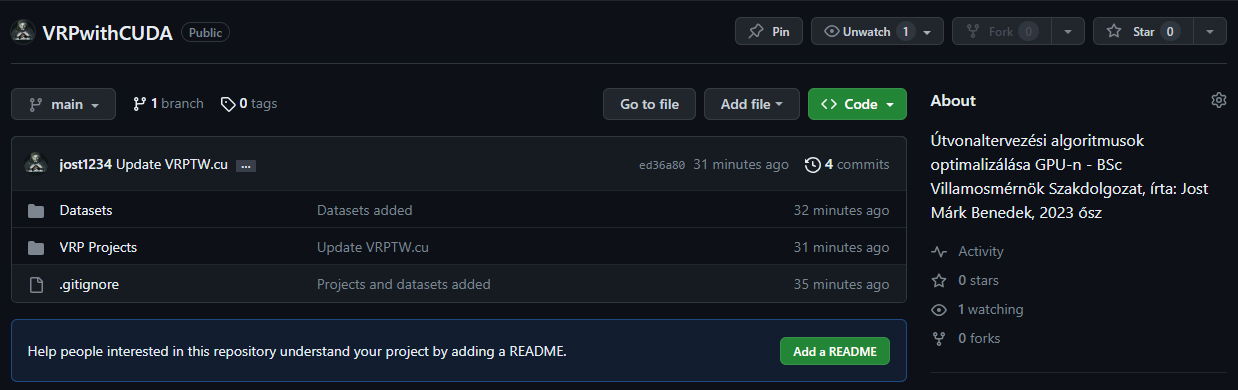
\includegraphics[width=150mm, keepaspectratio]{figures/github.png}
\caption{A dolgozat során készített CUDA projektek szabadon megtekinthetően githubon \href{https://github.com/jost1234/VRPwithCUDA}{IDE KATTINTVA}}
\label{fig:github} 
\end{figure}


%----------------------------------------------------------------------------
%\clearpage\section{A dolgozat során használt rövidítések}
%----------------------------------------------------------------------------

